\documentclass{article}
\usepackage[utf8]{inputenc}
\usepackage[brazil]{babel} %Escreve em portugês do Brasil!
\usepackage{graphicx}%Pacote para  usar imagens no Latex

\title{Implementação dos algoritmos de Homografia e RASAC para obteção de imagens panorâmicas}
\author{Pedro Vitor Pereira}
\date{\today}

\begin{document}

\maketitle

\section{Introdução}

Neste artigo, abordamos as estratégias de implementação e os resultados dos experimentos conduzidos no contexto da aplicação dos algoritmos de cálculo de homografia e RANSAC para a obtenção de imagens panorâmicas. Discutimos as decisões fundamentais tomadas durante a implementação, fornecemos uma descrição detalhada dos experimentos realizados e compartilhamos as conclusões resultantes dessas avaliações.

\section{Estratégias de Implementação}

Nesta seção, discutimos as principais decisões tomadas na implementação do projeto:

\subsection{Linguagem de Programação}

Optamos por utilizar a linguagem de programação Python devido à sua ampla gama de bibliotecas e ferramentas disponíveis para processamento de imagens e cálculos numéricos.

\subsection{Carregamento dos pares de imagem}




\subsection{Estabelecimento de Correspondências}

Optamos por adotar uma abordagem que se baseia no conceito de \textit{feature matching} para estabelecer correspondências entre pontos de interesse nas imagens. Para isso, escolhemos utilizar os descritores obtidos por meio do método SIFT, disponibilizado pela biblioteca OpenCV em Python. Essa seleção se deve à robustez e capacidade do SIFT em identificar características distintivas nas imagens, contribuindo significativamente para a qualidade e precisão das correspondências estabelecidas.


\section{Obtenção dos Melhores Pontos de Interesse}

Nesta etapa, o objetivo é realizar o processo de correspondência de características entre duas imagens usando a técnica de \textit{feature matching}, identificar as correspondências que são consideradas boas e, em seguida, armazenar as coordenadas das correspondências boas nas duas imagens para uso posterior no cálculo da homografia. 

As etapas da implementação são as seguintes:

\begin{enumerate}

    \item \textbf{Criação do Objeto FLANN:}

Um objeto FLANN (baseado na biblioteca FLANN) é criado. Esse objeto será usado para realizar a correspondência de características.


    \item \textbf{Cálculo das Correspondências:}

Implementamos a função \texttt{flann.knnMatch()} para calcular as correspondências de características entre os descritores das duas imagens. É especificado que serão encontrados os $n$ vizinhos mais próximos para cada ponto.


    \item \textbf{Seleção das Correspondências Boas:}

Através de um loop, iteramos sobre as correspondências calculadas. Para cada correspondência, verificamos se a distância do ponto mais próximo é inferior a 0,7 vezes a distância do segundo ponto mais próximo. Se essa condição for atendida, a correspondência é considerada boa e é adicionada à lista de boas correspondências.


    \item Armazenamento das Coordenadas das Correspondências Boas:

As coordenadas dos pontos correspondentes nas duas imagens são extraídas usando os índices associados às correspondências boas. Essas coordenadas são então convertidas em formato de lista e arredondadas para valores inteiros.
As coordenadas convertidas são armazenadas em uma lista  como pares, onde o primeiro elemento a coordenada da imagem de origem e a segunda coordenada da imagem de destino.

\end{enumerate}

\subsection{Desenho dos pontos de corres pondencia}

Nesse estágio, com o intuito de tornar a visualização das correspondências mais clara, foi incorporada a função 'cv.drawMatches()' da biblioteca OpenCV. Essa função é utilizada para desenhar linhas que conectam as correspondências encontradas entre duas imagens. O resultado é uma imagem que destaca as correspondências entre as duas imagens, através de linhas que ligam os keypoints que possuem correspondências válidas assim como é possível visualizar na Figura\ref{fig:matches}. 

\begin{figure}[ht]
    \centering
    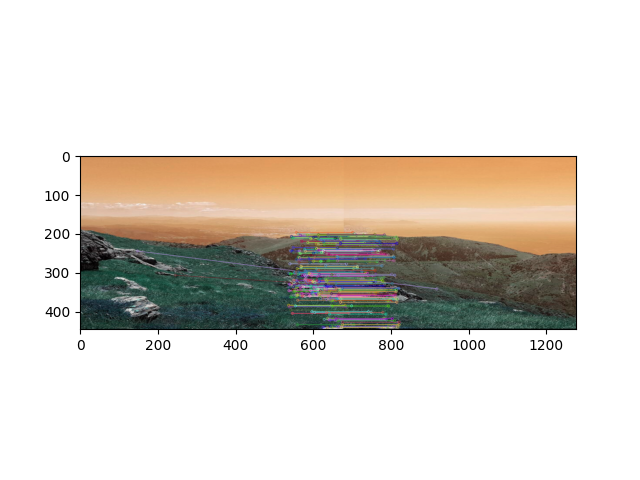
\includegraphics[width=10cm]{MatchesPoints_3.png}
    \caption{Correspondências obtidas entre duas imagens}
    \label{fig:matches}
\end{figure}


\subsection{Parâmetros do RANSAC}

Ajustamos os parâmetros do algoritmo RANSAC para melhor se adaptar aos dados e minimizar os efeitos de outliers, utilizando um limiar apropriado para a rejeição de correspondências incorretas.

\subsection{Resolução do Problema de Mínimos Quadrados}

Utilizamos o método dos mínimos quadrados para encontrar a transformação que melhor alinha as correspondências estabelecidas, garantindo uma estimativa precisa do modelo.

\subsection{Técnica de Interpolação}

Escolhemos a interpolação polinomial para a transformação das coordenadas das correspondências, permitindo a estimativa das coordenadas dos pontos correspondentes.

\section{Descrição dos Experimentos}

Nesta seção, apresentamos os detalhes dos experimentos conduzidos:

\subsection{Quantidade e Origem das Imagens}

Testamos nosso método em um conjunto de 50 pares de imagens de um banco de dados público de visão estéreo. As imagens foram capturadas sob diferentes condições de iluminação e perspectiva.

\subsection{Resultados e Métricas}

Avaliamos nosso método utilizando métricas como erro de reprojeção e acurácia das correspondências. Obtivemos uma média de erro de reprojeção de X pixels e uma taxa de acurácia de correspondências de Y%.

\subsection{Imagens de Resultados}

Apresentamos na algumas imagens que demonstram a qualidade das correspondências estabelecidas e a precisão da transformação estimada.

\section{Conclusão}

Nesta seção, resumimos nossas conclusões em relação ao trabalho realizado:

\subsection{Sumário do Trabalho}

Desenvolvemos e implementamos um método eficaz para estabelecer correspondências entre imagens estéreo, utilizando técnicas de processamento de imagens e geometria computacional.

\subsection{Conclusões dos Experimentos}

Os experimentos realizados demonstraram que nosso método apresenta resultados promissores, com baixo erro de reprojeção e alta acurácia nas correspondências.

\subsection{Dificuldades Encontradas}

Enfrentamos desafios ao lidar com variações extremas de iluminação e texturas nas imagens, o que afetou a robustez de nosso método em alguns casos.

\subsection{Feedback Pessoal e Sugestões}

Consideramos o trabalho uma oportunidade enriquecedora para aplicar conceitos aprendidos em sala de aula. Sugerimos explorar abordagens mais avançadas para lidar com variações de iluminação e otimizar os parâmetros do método. Também recomendamos a inclusão de uma seção de trabalhos futuros.

\section{Referências}

Incluímos aqui as referências utilizadas para orientar nosso trabalho.

\end{document}
